\documentclass[10pt,a4paper]{article}
%standard symbols
\usepackage{amssymb, amsmath, esint, mathrsfs, tipa}
%charts and tables
\usepackage{array, enumitem}
%graphics
\usepackage{graphicx}
%packages for float
\usepackage{wrapfig, placeins, float}
%specialized tools
\usepackage[americanvoltages,RPvoltages]{circuitikz}
%geometry
\usepackage[left=1.0cm, right=1.0cm, top=2.5cm]{geometry}
%code
\usepackage{listings}
%links
\usepackage{hyperref}

\setlength{\textfloatsep}{5pt plus 2pt minus 2pt}
\setlength{\floatsep}{5pt plus 2pt minus 2pt}

\begin{document}

%\tableofcontents

\section{Introduction}

These are a collection of personal notes on the optical data acquisition motherboard (ODMB), an circuit board used by the CMS CSC detectors.

\section{ODMB Firmware}

\subsection{Top Level}

The current ODMB firmware is largely split into two pieces The first is ODMB VME (MBV), which executes slow control such as sending commands to DCFEB or LVMB and changing ODMB settings. The second is ODMB CTRL (MBC), which executes fast control needed during data taking.

%\subsubsection{Clocks and QPLL}
The 160MHz and 40MHz clocks are produced by the qpll and are inputs to the FPGA. The \texttt{qpll\_reset} and \texttt{qpll\_autorestart} signals are held at `1'. The faster clocks (10 MHz, and 5 MHz) are then generated by a clock manager (MMCM) ip core from the 40 MHz clock. The slightly slower clocks (2.5 MHz, 5 MHz, 1.25 MHz, 0.625 MHz) are generated by dividing the 5 MHz clock with D flops. Finally, the very slow clocks (10 kHz and 1 kHz) are generated in a process with a counter.

%\subsubsection{VME Interface}
The VME interface consists of several signals, which go to the IC's on the ODMB that ultimately interface with the VME backplane. These signals are summarized in table \ref{tab:vmeinterface} with signals for the ICs between the FPGA and VME backplane listed below the double line. Inside the ODMB, most of these signals are sent to the \texttt{COMMAND\_MODULE} module in ODMB VME, which decodes the VME commands and send appropriate signals such as \texttt{STROBE}, \texttt{DEVICE}, and \texttt{COMMAND} to the ODMB VME devices. 

For more on VME protocol, see the section on the VME simulation. For more information about how ODMB deals with VME commands, reference the section on command modules. 

\begin{table}[H]
\begin{tabular}{|l|l|} \hline
Port& Description\\ \hline
\texttt{vme\_data}& VME data IO line, IOBUF controlled by \texttt{vme\_tovme (bar)}.\\ \hline
\texttt{vme\_addr}& Address from VME, given to \texttt{COMMAND\_MODULE}. The first 5 bits specify the slot(s) being addressed\\
                  & and the later 18 bits define the command given.\\ \hline
\texttt{vme\_am}& Address modifier from VME, given to \texttt{COMMAND\_MODULE}. This specifies the type of command being sent.\\ \hline
\texttt{vme\_gap}& Geographical address parity from VME, given to \texttt{COMMAND\_MODULE}. This bit is 1 if \texttt{vme\_ga} \\
                & has an even number of 1's and 0 otherwise. \\ \hline
\texttt{vme\_ga}& Geographical address from VME, given to \texttt{COMMAND\_MODULE}. These bits define the VME slot the\\
                 & board is currently connected to.\\ \hline
\texttt{vme\_as\_b}& Address strobe (bar) from VME, given to \texttt{COMMAND\_MODULE} and \texttt{VMECONFREGS}. This signal can \\
                   & be asserted after \texttt{vme\_addr} is ready to be read.\\ \hline
\texttt{vme\_ds\_b}& Data strobe (bar) from VME, given to \texttt{COMMAND\_MODULE}. These signals can be asserted after \\
                   & \texttt{vme\_data} is ready to be read or VCC is ready to read data. Each one corresponds to one byte \\
									 & on \texttt{vme\_data}\\ \hline
\texttt{vme\_sysfail\_b}& Sysfail (bar) signal from VME, given to \texttt{COMMAND\_MODULE}. Indicates a failure of the VME \\
                        & system.\\ \hline
\texttt{vme\_berr\_b}& Error (bar) signal from VME, given to \texttt{COMMAND\_MODULE}. Indicates an error in VME system and \\
                     & postpones any commands.\\ \hline
\texttt{vme\_iack\_b}& Interrupt acknowledge from VME, given to \texttt{COMMAND\_MODULE}. Commands should only be accepted \\
                     & while \texttt{IACK} is high, allowing VCC to interrupt commands by driving it low.\\ \hline
\texttt{vme\_lword\_b}& Load word signal from VME, given to \texttt{COMMAND\_MODULE}. Defines size of data transfers.\\ \hline
\texttt{vme\_write\_b}& write (bar) signal from VME, given to each device in \texttt{ODMB VME}. Indicates if the current \\
                      & command is a read or write command.\\ \hline
\texttt{vme\_dtack\_v6\_b}& Data acknowledge (bar) signal to VME, low when any \\
                 & device from ODMB VME issues a dtack.\\ \hline \hline
\texttt{vme\_tovme}& Output signal controlling direction of \texttt{vme\_data} both internally and on level translator ICs. \\
          & Not of \texttt{tovme\_b} from \texttt{COMMAND\_MODULE}\\ \hline
\texttt{vme\_doe\_b}& VME output enable (bar) signal from \texttt{COMMAND\_MODULE} for level translator ICs.\\ \hline
\end{tabular}
\caption{Signals in VME interface}
\label{tab:vmeinterface}
\end{table}

\subsection{VME Device 1: DCFEB JTAG and INITJAG}

The DCFEB JTAG device (cfebjtag.vhd) is the first device in the ODMB VME interface. This module is used to communicate with (x)(D)CFEBs via JTAG protocol (via the PPIB skew clear cables). The signals connecting to this interface are listed in table \ref{tab:cfebjtaginterface}. The VME command recognized by this device are shown in table \ref{tab:cfebjtagcommands}.

\begin{table}[H]
\begin{tabular}{|l|l|} \hline
Port& Description\\ \hline
\texttt{FASTCLK}& 40MHz clock from top level\\ \hline
\texttt{SLOWCLK}& 2.5MHz clock from top level. Called \texttt{clk\_s1} in odmb\_vme.vhd and top level and said \\
       &to be 10 MHz/0.625 MHz in incorrect comments\\ \hline
\texttt{RST}& Reset signal.\\ \hline
\texttt{DEVICE}& Signal to accept/ignore incoming commands/strobes. Should be connected to DEVICE(3) \\
      & output from \texttt{COMMAND\_MODULE}, which decodes VME commands- will be 1 for \\
			& VME commands 3XXX.\\ \hline 
\texttt{STROBE}& Signal that initiates command execution; generated by \texttt{COMMAND\_MODULE} \\
      & from VME strobe signals\\ \hline
\texttt{COMMAND}& Important bits of VME command (append ``00'' to end for full command)\\ \hline
\texttt{WRITER}& Unused, connected from \texttt{VME\_WRITE\_B}\\ \hline
\texttt{INDATA}& input directly from \texttt{VME\_DATA} line (through IOBUF)\\ \hline
\texttt{OUTDATA}& output multiplexed to \texttt{VME\_DATA} line (through IOBUF)\\ \hline
\texttt{DTACK}& acknowledge receipt of VME commands, OR'd with DTACKs from other devices \\
     & and sent back to VME. Active high\\ \hline
\texttt{INITJTAGS}& signal that resets module and sends signals to reset CFEB JTAG \\
         & state machine, generated when DONE received from (x)(D)CFEBs\\ \hline
\texttt{TCK}& JTAG output to (x)(D)CFEB, one per (x)(D)CFEB\\ \hline
\texttt{TDI}& JTAG output to (x)(D)CFEB, common to all (x)(D)CFEBs\\ \hline
\texttt{TMS}& JTAG output to (x)(D)CFEB, common to all (x)(D)CFEBs\\ \hline
\texttt{FEBTDO}& JTAG input from (x)(D)CFEB, one per (x)(D)CFEBs\\ \hline
\texttt{LED}& DEBUG output\\ \hline
\texttt{DIAGOUT}& DEBUG output\\ \hline
\texttt{CSP\_LVMB\_LA\_CTRL}& Unused\\ \hline
\end{tabular}
\caption{Ports for CFEBJTAG device}
\label{tab:cfebjtaginterface}
\end{table}

\begin{table}[H]
\begin{tabular}{|l|l|} \hline
COMMAND& Description\\ \hline
\texttt{W 1Y00}& Shift data, no TMS header or tailer.\\ \hline
\texttt{W 1Y04}& Shift data, preceded by TMS header.\\ \hline
\texttt{W 1Y08}& Shift data, followed by TMS tailer.\\ \hline
\texttt{W 1Y0C}& Shift data, preceded by TMS header and followed by TMS tailer.\\ \hline
\texttt{R 1014}& Read TDO register.\\ \hline
\texttt{W 1018}& Reset JTAG to idle.\\ \hline
\texttt{W 1Y1C}& Shift data, preceded by TMS header and followed by TMS tailer. (Legacy)\\ \hline
\texttt{W 1020}& Select DCFEB (1 bit per DCFEB).\\ \hline
\texttt{R 1024}& Read selected DCFEBs.\\ \hline
\texttt{W 1Y30}& Shift instruction, no TMS header or tailer.\\ \hline
\texttt{W 1Y34}& Shift instruction, preceded by TMS header.\\ \hline
\texttt{W 1Y38}& Shift instruction, followed by TMS tailer.\\ \hline
\texttt{W 1Y3C}& Shift instruction, preceded by TMS header and followed by TMS tailer.\\ \hline
\texttt{W 1Y48}& Shift instruction, followed by special TMS tailer.\\ \hline
\texttt{W 1Y4C}& Shift instruction, preceded by TMS header and followed by special TMS tailer.\\ \hline
\end{tabular}
\caption{CFEB JTAG accepted commands}
\label{tab:cfebjtagcommands}
\end{table}

%\subsubsection{TCK generation}
When a STROBE signal is received and there is an appropriate VME command, a LOAD signal is generated, which then generates a BUSY signal. While BUSY is high, the global TCK clock \texttt{TCK\_GLOBAL} will run with the \texttt{SLOWCLK}. Previous versions of development firmware would give `ghost strobe' signals, which cause TCK to run with TMS/TDI set to a constant 0. This may result in strange commands being sent to the (x)(D)CFEBs.

%\subsubsection{TMS generation}
The TMS signals are generated by loops of sequentially connected D flops. By using FDC(E) and FDP(E) flops, certain sequences of 1's and 0's are achieved in order to control the JTAG state machine. The FD flops from the \texttt{Latches\_Flipflops} package are found not to work on the KCU105 evaluation board and were replaced with the equivalent UNISIM components. Furthermore, the CB4CE and SR16LCE functions from the \texttt{Latches\_Flipflops} package did not defaultly work on the KCU105 evaluation board, and their implementation was slightly tweaked to nest conditions rather than AND'ing them. It is unclear why this changes behavior.

%\subsubsection{DCFEB done in top level}
The \texttt{INITJTAG} signal is generated after receiving DONE from the (x)(D)CFEBs. The signal \texttt{pon\_rst\_reg} is initialized to a particular value when \texttt{PLL\_LOCK} is on (when ODMB is reset) and after a few clock cycles, \texttt{pon\_reset} becomes '1', which sets the FSM \texttt{done\_current\_state} to \texttt{DONE\_LOW}. When the \texttt{DONE} for an (x)(D)CFEB becomes `1', the \texttt{done\_current\_state} is set to \texttt{DONE\_COUNTING}, which generates \texttt{dcfeb\_done\_pulse} before setting the FSM to \texttt{DONE\_IDLE}. All the \texttt{dcfeb\_done\_pulse}'s are OR'd together and converted to a pulse to generate \texttt{INITJTAG}. Perhaps this logic could be moved from the top level to inside of cfebjtag.vhd. Note that the FSM counter runs on the 10 kHz clock, which is just generated in a process somewhere and not BUFG'd. 

%SHDATA and DONEDATA
When \texttt{BUSY} is asserted, but the header is not being shifted (\texttt{IHEADEN}=\texttt{DHEADEN}=0) and \texttt{DONEDATA} is false, \texttt{SHDATA(X)} will be asserted. When \texttt{LOAD} is asserted, the length of the JTAG command (bits 9 down to 6) is loaded into a 4 bit counter. Once \texttt{SHDATA} is asserted, the counter counts down with \texttt{SLOWCLK} until 0. When the counter is zero and a \texttt{SLOWCLK} clock edge comes, \texttt{DONEDATA}(0) is asserted, and on the next clock edge \texttt{DONEDATA}(1) is asserted. 

%OUTDATA generation
When data is being read (\texttt{SHDATA(X)}=1), \texttt{TDO} from the selected DCFEB is shifted into \texttt{Q\_OUTDATA} using a 16 bit shift register. When a read command (1014) is received, along with a strobe and \texttt{BUSY} is not asserted, \texttt{RTDODK} will be asserted. This will present \texttt{Q\_OUTDATA} to the output port.

%DTACK
\texttt{DTACK} may be asserted when one of several conditions is met. For a `read selected CFEB' command, \texttt{DTACK} will be asserted when the data is ready to read. For a read command, \texttt{DTACK} will be asserted when \texttt{RTDODK} is asserted. For a reset command, \texttt{DTACK} will be asserted when \texttt{RESETDONE} is asserted. Finally, if \texttt{DATASHIFT} or \texttt{INSTSHIFT} is asserted but \texttt{BUSY} has been low for four \texttt{SLOWCLK} cycles, \texttt{DTACK} will be asserted.
%Similarly, when issuing a read command, \texttt{DTACK} will be asserted when the data is ready to be read.

\subsection{VME Device 3: VMEMON (A.K.A. ODMB/DCFEB Control)}

The VMEMON device (vmemon.vhd) is the third device in the ODMB VME interface. This module is used to set various configuration registers and read back various data registers. The signals connecting to this interface are listed in table \ref{tab:vmemoninterface}. %The VME command recognized by this device are shown in table \ref{tab:vmemoncommands}.

\begin{table}[H]
\begin{tabular}{|l|l|} \hline
Port& Description\\ \hline
\texttt{CLK40}& 40MHz clock from top level\\ \hline
\texttt{SLOWCLK}& 2.5MHz clock from top level. Called \texttt{clk\_s1} in odmb\_vme.vhd and top level and said \\
       &to be 10 MHz/0.625 MHz in incorrect comments\\ \hline
\texttt{RST}& Reset signal.\\ \hline
\texttt{DEVICE}& Signal to accept/ignore incoming commands/strobes. Should be connected to DEVICE(3) \\
      & output from \texttt{COMMAND\_MODULE}, which decodes VME commands- will be 1 for \\
			& VME commands 3XXX.\\ \hline 
\texttt{STROBE}& Signal that initiates command execution; generated by \texttt{COMMAND\_MODULE} \\
      & from VME strobe signals\\ \hline
\texttt{COMMAND}& Important bits of VME command (append ``00'' to end for full command)\\ \hline
\texttt{WRITER}& Indicates direction of read/write commands, connected from \texttt{VME\_WRITE\_B}\\ \hline
\texttt{INDATA}& input directly from \texttt{VME\_DATA} line (through IOBUF)\\ \hline
\texttt{OUTDATA}& output multiplexed to \texttt{VME\_DATA} line (through IOBUF)\\ \hline
\texttt{DTACK}& acknowledge receipt of VME commands, OR'd with DTACKs from other devices \\
     & and sent back to VME. Active high\\ \hline
\texttt{DCFEB\_DONE}& Vector of \texttt{DONE} signals directly from PPIB.\\ \hline
\texttt{QPLL\_LOCKED}& QPLL lock signal directly from QPLL.\\ \hline
\texttt{OPT\_RESET\_PULSE}& output signal that generates a pulse in the reset signal to the GTX/GTH modules.\\ \hline
\texttt{L1A\_RESET\_PULSE}& output signal that generates a reset signal to the L1A counter (in ODMB CTRL)\\
                          &  and CFEB RESYNC.\\ \hline
\texttt{FW\_RESET}& output signal that generates a general soft reset (to ODMB CTRL, BPI interface, etc.).\\ \hline
\texttt{REPROG\_B}& output hard reset output signal to CFEBs.\\ \hline
\texttt{TEST\_INJ}& output sent to \texttt{TEST\_CCBINJ} port of ODMB CTRL. \\ \hline
\texttt{TEST\_PLS}& output sent to \texttt{TEST\_CCBPLS} port of ODMB CTRL. \\ \hline
\texttt{TEST\_PED}& output sent to \texttt{TEST\_CCBPED} port of ODMB CTRL. \\ \hline
\texttt{TEST\_BC0}& output sent to PPIB (output \texttt{DCFEB\_BC0}) after delay. \\ \hline
\texttt{TEST\_LCT}& output that generates an L1A in the top level. \\ \hline
\texttt{OTMB\_LCT\_RQST}& output sent to OTMB (output \texttt{LCTRQST}(1)) \\ \hline
\texttt{OTMB\_EXT\_TRIG}& output sent to OTMB (output \texttt{LCTRQST}(2)) \\ \hline
\texttt{MASK\_PLS}& output masks to '0' signal from ODMB CTRL to DCFEB pulses (output \texttt{DCFEB\_INJPLS}\\ 
                  & and \texttt{DCFEB\_EXTPLS}) \\ \hline
\texttt{MASK\_L1A}& output masks to '0' DCFEB-bound signals \texttt{DCFEB\_L1A} and \texttt{DCFEB\_L1A\_MATCH} \\ \hline
\texttt{MASK\_L1A}& output masks to '0' DCFEB-bound signals \texttt{DCFEB\_L1A} and \texttt{DCFEB\_L1A\_MATCH} \\ \hline
\texttt{TP\_SEL}& output that selects what signals are on which test ODMB points \\ \hline
\texttt{MAX\_WORDS\_DCFEB}& output that sets number of invalid words received from a DCFEB before it is considered bad\\ \hline
\texttt{ODMB\_CTRL}& output, control bits for ODMB, see table \ref{tab:odmbctrlbits}\\ \hline
\texttt{ODMB\_DATA\_SEL}& output, selects configuration data to read from top level, see manual.\\ \hline
\texttt{ODMB\_DATA}& input from top level with configuration data to read\\ \hline
\texttt{TXDIFFCTRL}& output signal that controls voltage swings on the GTX/GTH modules.\\ \hline
\texttt{LOOPBACK}& output signal to GTX/GTH modules needed for loopback tests.\\ \hline
\end{tabular}
\caption{Ports for VMEMON device}
\label{tab:vmemoninterface}
\end{table}

\begin{table}[H]
\begin{tabular}{|l|l|} \hline
Bits& Description\\ \hline
5 downto 0& calibration mode, sent to ODMB CTRL (1: generate L1A with each pulse)\\ \hline
6& Unused \\ \hline
7& data multiplexer (0: real data from ALCT/DCFEB/OTMB, 1: dummy data)\\ \hline
8& ODMB soft reset, only used for reference\\ \hline
9& trigger multiplexer, used various places (0: external triggers, 1: internal triggers)\\ \hline 
10& LVMB multiplexer, sent to LVMB\_MUX module (0: real LVMB, 1: dummy LVMB)\\ \hline
11& Mask L1A's/L1A Matches, only used for reference \\ \hline
12& Mask L1A's/L1A Matches, only used for reference \\ \hline
13& Pedestal mode, sent to ODMB CTRL (1: L1A\_MATCH sent with each L1A)\\ \hline 
14& OTMB Pedestal mode, sent to ODMB CTRL (1: L1A\_MATCH sent with each L1A)\\ \hline
15& Unused \\ \hline	
\end{tabular}
\caption{Bits in \texttt{ODMB\_CTRL\_REG}}
\label{tab:odmbctrlbits}
\end{table}

\subsection{VME Device 4: VMECONFREGS (Configuration Registers)}

\begin{table}[H]
\begin{tabular}{|l|l|} \hline
Port& Description\\ \hline
\texttt{CLK40}& 40MHz clock from top level.\\ \hline
\texttt{CLK}& 2.5MHz clock from top level.\\ \hline
\texttt{RST}& Reset signal.\\ \hline
\texttt{DEVICE}& Signal to accept/ignore incoming commands/strobes. Should be connected to DEVICE(4) \\
      & output from \texttt{COMMAND\_MODULE}, which decodes VME commands- will be 1 for \\
			& VME commands 4XXX.\\ \hline 
\texttt{STROBE}& Signal that initiates command execution; generated by \texttt{COMMAND\_MODULE} \\
      & from VME strobe signals\\ \hline
\texttt{COMMAND}& Important bits of VME command (append ``00'' to end for full command)\\ \hline
\texttt{WRITER}& Indicates direction of read/write commands, connected from \texttt{VME\_WRITE\_B}\\ \hline
\texttt{VME\_AS\_B}& VME address strobe, checked when from \texttt{VME\_AS\_B} (why?)\\ \hline
\texttt{INDATA}& input directly from \texttt{VME\_DATA} line (through IOBUF)\\ \hline
\texttt{OUTDATA}& output multiplexed to \texttt{VME\_DATA} line (through IOBUF)\\ \hline
\texttt{LCT\_L1A\_DLY}& outputs LCT L1A delay register (delays CLCT), used in ODMB CTRL and triggers\\ \hline
\texttt{CABLE\_DLY}& outputs ALCT push delay register, used to delay L1A(\_MATCH)s, BC0s, and RESYNCs \\
                   & to DCFEBs\\ \hline
\texttt{OTMB\_PUSH\_DLY}& outputs OTMB push delay register (\texttt{OTMBDAV} is delayed by\\
                        & \texttt{push\_delay}-\texttt{OTMB\_PUSH\_DLY}), used in ODMB CTRL \\
												& and triggers\\ \hline
\texttt{ALCT\_PUSH\_DLY}& outputs ALCT push delay register (\texttt{ALCTDAV} is delayed by  \\
                        & \texttt{push\_delay}-\texttt{ALCT\_PUSH\_DLY}), used in ODMB CTRL and \\
												& triggers\\ \hline
\texttt{BX\_DLY}& outputs bunch crossing delay register, used in ODMB CTRL\\ \hline
\texttt{INJ\_DLY}& outputs INJ pulse delay register (delay from CCB calibration 1 pulse to DCFEB INJ \\
                 & pulse), used in ODMB CTRL\\ \hline
\texttt{EXT\_DLY}& outputs EXT pulse delay register (delay from CCB calibration 2 pulse to DCFEB EXT \\
                 & pulse), used in ODMB CTRL\\ \hline
\texttt{CALLCT\_DLY}& outputs CALLCT pulse delay register (delay from DCFEB INJ/EXT pulse to L1A), \\
                 & used in ODMB CTRL\\ \hline
\texttt{ODMB\_ID}& outputs ODMB unique ID from TMR const registers loaded from PROM, used by LVDBMON,\\
                 & ODMBJTAG, and DCFEB I/O to change behavior for different ODMB boards\\ \hline
\texttt{NWORDS\_DUMMY}& outputs number of words to generate to fake DCFEB and OTMB/ALCT\\ \hline
\texttt{KILL}& outputs whether to kill DCFEBs, ALCT, and OTMB, used various locations including ODMB \\
             & CTRL\\ \hline
\texttt{CRATEID}& outputs crate ID, used in ODMB CTRL when sending packets to DDU\\ \hline
\texttt{BPI\_CFG\_UL\_PULSE}& input from BPI\_PORT, indicates upload of CFG registers to PROM\\ \hline
\texttt{BPI\_CFG\_DL\_PULSE}& input from BPI\_PORT, indicates download of CFG registers from PROM \\
                            & (?) (unused)\\ \hline
\texttt{BPI\_CONST\_UL\_PULSE}& input from BPI\_PORT, indicates upload of const registers to PROM\\ \hline
\texttt{BPI\_CONST\_DL\_PULSE}& input from BPI\_PORT, indicates download of const registers form PROM \\
                              & (?) (unused)\\ \hline
\texttt{CHANGE\_REG\_DATA}& input from top level, contains current kill/bad DCFEBs\\ \hline
\texttt{CHANGE\_REG\_INDEX}& input from top level, is 7 if any DCFEBs are marked bad or good, 16 \\
                           & otherwise\\ \hline
\texttt{CC\_CFG\_REG\_IN}& input from BPI\_CTRL (PROM) used to load CFG and const registers\\ \hline
\texttt{BPI\_CONST\_BUSY}& input from BPI\_CONST\_CONTROLLER checked when writing to const registers\\ \hline
\texttt{CC\_CONST\_REG\_WE}& input from BPI\_CONST\_CONTROLLER checked when writing to const\\
                           & registers\\ \hline
\texttt{BPI\_CONST\_REGS}& output used to write to BPI\_CONST\_CONTROLLER\\ \hline
\texttt{BPI\_CFG\_BUSY}& input from BPI\_CFG\_CONTROLLER checked when writing to CFG registers\\ \hline
\texttt{CC\_CFG\_REG\_WE}& input from BPI\_CFG\_CONTROLLER checked when writing to CFG registers\\ \hline
\texttt{BPI\_CFG\_REGS}& output used to write to BPI\_CFG\_CONTROLLER\\ \hline
\end{tabular}
\caption{Ports on VMECONFREGS device}
\label{tab:vmeconfregsinterface}
\end{table}

%402C command not documented

\subsection{ODMB VME: Command Module}

The command module (command.vhd) is a helper device in the ODMB VME interface responsible for decoding the signals received from the VME backplane. The signals connecting to this interface are listed in table \ref{tab:commandinterface}.

\begin{table}[H]
\begin{tabular}{|l|l|} \hline
Port& Description\\ \hline
\texttt{FASTCLK}& 40MHz clock from top level\\ \hline
\texttt{SLOWCLK}& 2.5MHz clock from top level\\ \hline
\texttt{GA}& VME geographical address from \texttt{VME\_GA} and \texttt{VME\_GAP} (\texttt{GA(5)} should be \texttt{VME\_GAP})\\ \hline
\texttt{ADR}& VME address from \texttt{VME\_ADDR}\\ \hline
\texttt{AM}& VME address modifier from \texttt{VME\_AM}\\ \hline
\texttt{AS}& VME address strobe (bar) from \texttt{VME\_AS\_B}\\ \hline
\texttt{DS0}& Lower bit of VME data strobe (bar) from \texttt{VME\_DS\_B(0)}\\ \hline
\texttt{DS1}& Upper bit of VME data strobe (bar) from \texttt{VME\_DS\_B(1)}\\ \hline
\texttt{LWORD}& VME load word (bar) from \texttt{VME\_LWORD\_B}\\ \hline
\texttt{WRITER}& VME write (bar) signal from \texttt{VME\_WRITE\_B}\\ \hline
\texttt{IACK}& VME interrupt acknowledge (bar) from \texttt{VME\_IACK\_B}\\ \hline
\texttt{BERR}& VME error (bar) signal from \texttt{VME\_BERR\_B}\\ \hline
\texttt{SYSFAIL}& VME SYSFAIL (bar) signal from \texttt{VME\_SYSFAIL\_B}\\ \hline
\texttt{TOVME\_B}& signal controlling \texttt{VME\_DATA} IOBUF at top level and output as (barred) \texttt{VME\_TOVME}\\ \hline
\texttt{DOE\_B}& VME output enable (bar) output as \texttt{VME\_DOE\_B}\\ \hline
\texttt{DEVICE}& each of 10 bits indicates to ODMB VME device if it is selected\\ \hline
\texttt{STROBE}& signal sent to ODMB VME devices to indicate command ready\\ \hline
\texttt{COMMAND}& decoded VME command sent to each ODMB VME device\\ \hline
\texttt{ADRS}& used to multiplex \texttt{VME\_DATA\_OUT} from the various devices\\ \hline
\texttt{DIAGOUT}& for debugging\\ \hline
\texttt{LED}& for debugging\\ \hline
\end{tabular}
\caption{Signals in command module device}
\label{tab:commandinterface}
\end{table}

This device records the values of \texttt{AM} and \texttt{ADDR} (as \texttt{AMS} and \texttt{ADDR\_INNER} as they are when \texttt{AS} goes low (when \texttt{AS} is high, the internal values directly reflect the current values provided by the VME backplane). The command module interprets these to generate \texttt{DEVICE} and \texttt{COMMAND}, which are sent to the ODMB VME modules to interpret.

The command module checks that \texttt{GAP} matches the parity of the number of zeroes of \texttt{GA} and saves the result as \texttt{VALIDGA/GOODGA}. It checks AMS, and the ODMB only responds to commands with the format ``111XYZ'' where Y$\neq$Z and for which LWORD is 1. It also checks for commands it should respond to, which either (1) are addressed to this particular slot and have \texttt{ADDR}(23 downto 19) matching \texttt{GA}, (2) are broadcasted and have \texttt{ADDR}(23 downto 19) as ``11111'', or (3) \texttt{GA} is ``00000'', which indicates the \texttt{GA} pins are not functional. If the ODMB should respond to a particular commnad, \texttt{BOARDENB} is set high. Finally, this module checks \texttt{SYSFAIL} and \texttt{IACK}, which should both be high for the ODMB to respond to a command. When \texttt{GAP} is valid, \texttt{AM} and \texttt{LWORD} are appropriate, the command is for the ODMB, and no failures or interrupts are detected, the command module assigns \texttt{tovme} based on \texttt{write}. When the above conditions are met and both \texttt{DS0} and \texttt{DS1} are low, it generates the signal \texttt{strobe} and sends it to the ODMB VME modules to prompt action.

\subsection{ODMB CTRL Device 1: CALIBTRG}

This device generates calibration triggers when prompted by the CCB. It is used during STEP testing and calibration, but not during standard data taking. 

\begin{table}[H]
\begin{tabular}{|l|l|} \hline
Port& Description\\ \hline
\texttt{CMSCLK}& 40MHz clock input from top level\\ \hline
\texttt{CLK80}& 80MHz clock input from top level\\ \hline
\texttt{RST}& reset signal input from top level\\ \hline
\texttt{PLSINJEN}& pulse enable, input from ODMB CTRL, which just oscillates on and off when enabled\\ \hline
\texttt{CCBPLS}& input from ODMB CTRL to generate PLSBACK and INJPLS\\ \hline
\texttt{CCBINJ}& input from ODMB CTRL to generate INJBACK and INJPLS\\ \hline
\texttt{FINJ}& input from VMEMON to generate test INJBACK and INJPLS\\ \hline
\texttt{FPLS}& input from VMEMON to generate test PLSBACK and INJPLS\\ \hline
\texttt{FPED}& input from VMEMON to generate test pedestal output (unused)\\ \hline
\texttt{PRELCT}& input that generates PLS, tied to 0\\ \hline
\texttt{PREGTRG}& unused input, tied to 0\\ \hline
\texttt{INJ\_DLY}& input from VMECONFREGS indicating delay between CCB\_CAL1 and INJ\_PLS\\ \hline
\texttt{EXT\_DLY}& input from VMECONREGS indicating delay between CCB\_CAL0 and EXT\_PLS (PLSBACK)\\ \hline
\texttt{CALLCT\_DLY}& input from VMECONFREGS indicating delay between PLS and L1A\\ \hline
\texttt{LCT\_L1A\_DLY}& input from VMECONFREGS indicating delay between preLCT and L1A\\ \hline
\texttt{RNDMPLS}& unused input, tied to 0\\ \hline
\texttt{RNDMGTRG}& unused input, tied to 0\\ \hline
\texttt{PEDESTAL}& unused output\\ \hline
\texttt{CAL\_GTRG}& output trigger sent to CAL\_L1A port of TRGCNTRL\\ \hline
\texttt{CALLCT}& output LCT sent to CAL\_LCT port of TRGCNTRL\\ \hline
\texttt{INJBACK}& output sent to DCFEB\_INJPULSE\\ \hline
\texttt{PLSBACK}& output sent to DCFEB\_EXTPULSE\\ \hline
\texttt{LCTRQST}& unused output\\ \hline
\texttt{INJPLS}& unused output\\ \hline
\end{tabular}
\caption{Signals in CALIBTRG device}
\label{tab:calibtriginterface}
\end{table}

\subsection{VME Simulation}

The basic functionality of a single command sent by the VME protocol is described by the following steps.

\begin{enumerate}
\item Drive status signals like AM and LWORD
\item Set valid ADDRESS and drive IACK high
\item After at ADDRESS is valid for at least 35 ns, can drive AS low to indicate ADDRESS is ready to read
\item Wait until DTACK and BERR high, then set valid WRITE and DATA if applicable
\item After DATA is valid for at least 35 ns or VCC is ready to read data, can drive DS low to indicate DATA is ready to read/be read. Note that DTACK should be released for DS to be driven
\item When slave (ODMB) has read VME signals, it drives DTACK low
\item Once DTACK has been low for 10 ns, master (VCC) can stop driving its signals (AS, DS, IACK, etc.)
\item At some later point, ODMB can stop driving DTACK
\end{enumerate}

Note that the VME simulation currently differs from the above steps in that it waits for ODMB to release DTACK before it releases IACK. 

The VME simulation is described by the state machine in figure \ref{fig:vmestatemachine}. Although the time-out functionality works in simulation, it works inconsistently on the KCU105 evaluation board. for more information on the VME protocol, see \href{http://www.interfacebus.com/Design_Connector_VME.html}{VME Reference}.

\begin{figure}[H]
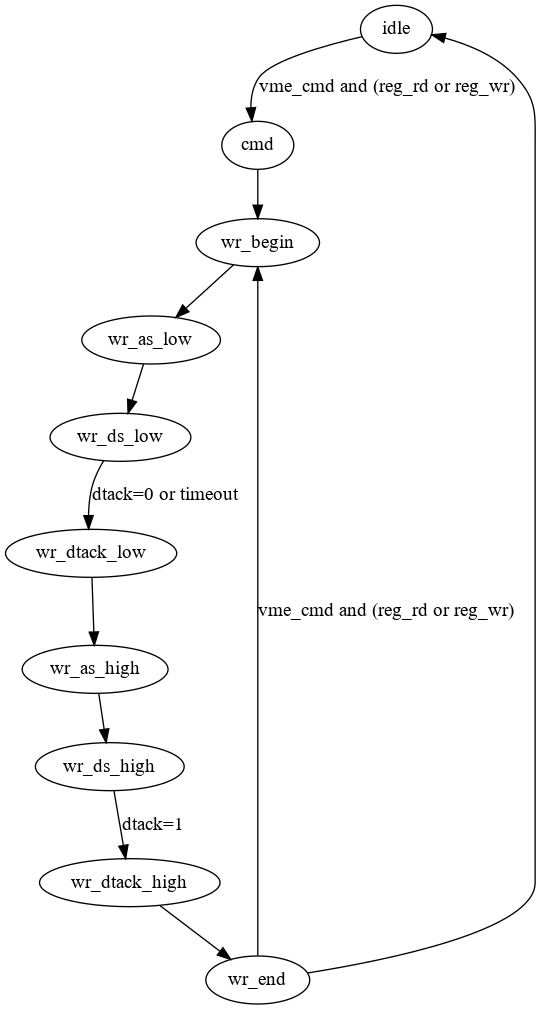
\includegraphics[width= 0.4 \textwidth]{figures/vmestates.png}
\caption{Simulated VME state machine}
\label{fig:vmestatemachine}
\end{figure}

\subsection{DCFEB Simulation}

\texttt{dcfeb\_v6.vhd} contains a simulation of both DCFEB JTAG and fake-data generation functionality. The \texttt{bgb\_scan\_emulator} module directly takes in the JTAG inputs TMS and TDI and decodes the input JTAG signals. User commands (``\texttt{0x3C2}'') are decoded by the module \texttt{instr\_decode}, which then outputs a signal called \texttt{FSEL}. This goes to the modules that execute the different user commands such as \texttt{usr\_wr\_reg}, which handles ADC mask write command \texttt{0x0c}, \texttt{user\_cap\_reg}, which handles the BPI status command \texttt{0x17}, and the new \texttt{user\_counter\_reg}, which handles read counter commands \texttt{0x3B} and \texttt{0x3C}.

%\bibliography{writeup}
%\bibliographystyle{plain}

\end{document}
